\documentclass{prova}

\usepackage{amsmath}
\usepackage{amsfonts}

\setlength{\textheight}{25cm}

\renewcommand{\sin}{\,\mbox{sen}\,}
\newcommand{\ds}{\displaystyle}

\professor{Prof.\@ Adriano Barbosa}
\disciplina{C\'alculo Diferencial e Integral III}
\avaliacao{P2}
\curso{Engenharia Mecânica}
\data{25/05/2021}

\begin{document}
	\cabecalho{5}  % o numero 5 indica a qnt de quadros na tabela de nota

    \textbf{Todas as respostas devem ser justificadas.}

    \begin{questionario}
        \q{Dada a região $R$:}
            \begin{figure}[h]
                \centering
                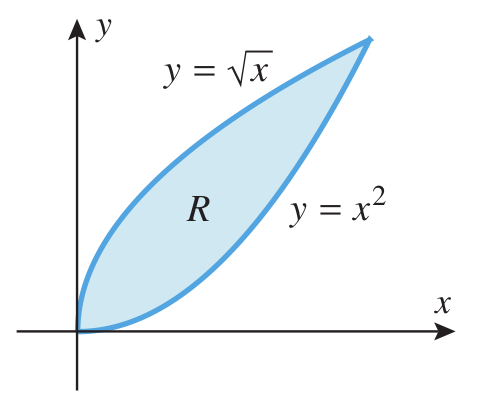
\includegraphics[width=0.25\textwidth]{grafico.png}
            \end{figure}
            \begin{questionario}
                \qq{Determine os limites de integração das integrais abaixo:}
                    \[\int\int_R f(x,y)\ dA = \int\ \int\ f(x,y)\ dx dy\]
                    \[\int\int_R f(x,y)\ dA = \int\ \int\ f(x,y)\ dy dx\]
                \qq{Calcule a área da região $R$.}
            \end{questionario}
        \q{Calcule a integral utilizando coordenadas polares
            $\ds\int_0^1\int_0^{\sqrt{1-y^2}} \cos{(x^2+y^2)}\ dxdy$.}
        \q{Calcule o volume do sólido $E$ limitado pela calota de esfera
            $z=\sqrt{25-x^2-y^2}$, pelo plano $z=0$ e pelo cilindro $x^2+y^2=9$.}
            \begin{figure}[h]
                \centering
                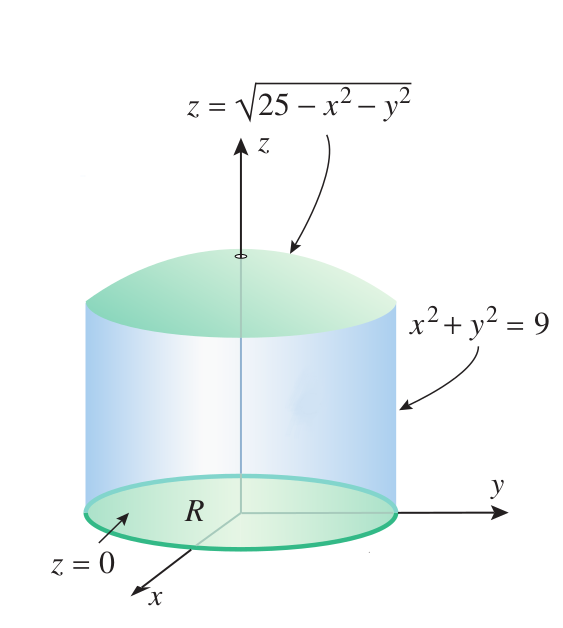
\includegraphics[width=0.3\textwidth]{cilindro.png}
            \end{figure}
        \q{Dado o campo $\ds F(x,y) = \left(e^x \ln{y} - \frac{e^y}{x},
            \frac{e^x}{y} - e^y \ln{x}\right)$:}
            \begin{questionario}
                \qq{Determine de $F$ é conservativo.}
                \qq{Calcule $\ds\int_C F\cdot dr$, onde $C: r(t)=(t^2, t^3),
                    t\in[1,2]$.}
            \end{questionario}
        \q{Sejam $F(x,y) = (x^2+y, y^2+2x)$ e $C$ a borda da região limitada
            pelas parábolas $y=x^2$ e $x=y^2$ orientada positivamente.
            Calcule $\ds\int_C F\cdot dr$. [Dica: use o exercício 1.]}
    \end{questionario}
\end{document}
